%==============================================================================%
%  Dependent Origination: A Mathematical Formalization of Interdependence     %
%  in Quantum and Cosmological Systems                                        %
%==============================================================================%
\documentclass[%
  prd,
  twocolumn,
  10pt,
  nofootinbib,
  tightenlines,
  showkeys
]{revtex4-2}

%--- Encoding & Micro-Typography ------------------------------------------------
\usepackage[T1]{fontenc}
\usepackage[utf8]{inputenc}
\usepackage{microtype}

%--- Mathematics ----------------------------------------------------------------
\usepackage{amsmath,amssymb}

%--- Graphics & Diagrams --------------------------------------------------------
\usepackage{graphicx}
\usepackage{tikz}
  \usetikzlibrary{positioning}

%--- Hyperlinks & Clever References --------------------------------------------
\usepackage[colorlinks=true,linkcolor=blue,citecolor=blue,urlcolor=blue]{hyperref}
\usepackage[nameinlink]{cleveref}

%--- Float spacing tweaks -------------------------------------------------------
\setlength{\textfloatsep}{8pt plus 2pt minus 2pt}
\setlength{\floatsep}{8pt plus 2pt minus 2pt}

%==============================================================================%
%                              Start of Document                              %
%==============================================================================%
\begin{document}

\title{Dependent Origination:\\
A Mathematical Formalization of Interdependence in Quantum and Cosmological Systems}

\author{Andrei Preece}
\author{Boris Batenin}
\affiliation{Independent Research, Berlin, Germany}

\date{June 27, 2025}

\begin{abstract}
We present a rigorous mathematical formalization of \emph{dependent origination}
(Pratītyasamuṭpāda), the principle taught by Buddha Shakyamuni, as a universal
framework for causality in quantum and cosmological contexts. By excluding the alternatives
of self-causation, external causation, dual causation, and causeless emergence, we show
that only an interdependent-conditions model remains logically and empirically viable.
We employ vacuum wave-functions, discrete-time Markov chains, and a fractal nesting
of spacetime spheres (golden-ratio scaled) to capture probabilistic interdependence.
Two TikZ diagrams—a directed acyclic graph and a fractal nesting—visualize
the causal flow without disturbing text flow. Finally, we derive testable predictions
for gravitational lensing, CMB anomalies, and LHC bounds.
\end{abstract}

\keywords{Dependent origination; Causality; Markov chains; Fractal geometry;
Quantum cosmology}

\maketitle

%-------------------------------------------------------------------------------
\section{Introduction}
Dependent origination posits that no phenomenon exists in isolation: each arises
from mutually sustaining conditions. Rejecting self-causation, purely external
causation, dual causation, and causeless emergence, we reinterpret this ancient
principle in modern physics. Our framework integrates quantum vacuum fluctuations,
Markov-chain transition dynamics, and golden-ratio fractal embeddings to yield
a coherent, testable model.

%-------------------------------------------------------------------------------
\section{Models of Causation}\label{sec:causation}
We consider four archetypal models:
\begin{enumerate}
  \item \emph{Self-Causation}: A phenomenon produces itself (infinite regress).
  \item \emph{External Causation}: A phenomenon is entirely sourced externally
        (violates relationality).
  \item \emph{Dual Causation}: Combines self and external causation (inconsistent).
  \item \emph{Non-Causation}: Spontaneous emergence (violates conservation).
\end{enumerate}
Each fails logical or empirical consistency, leaving only an interdependent network.

%-------------------------------------------------------------------------------
\section{Formalism}\label{sec:formalism}

\subsection{Vacuum Wave Function}
Define
\begin{subequations}
\begin{align}
  \Psi_\text{void} &= \sum_i \Psi_i,\\
  \Psi_\text{void} &= 0,
\end{align}
\end{subequations}
where each $\Psi_i$ is a vacuum fluctuation state (energy, field-mode, etc.).
The sum-to-zero enforces overall conservation.

\subsection{Markov-Chain Causality}
Let $\{X_n\}$ be a discrete-time chain with
\begin{equation}
  P(X_{n+1}=x\mid X_n=x_n,\dots,X_0=x_0)
  =P(X_{n+1}=x\mid X_n=x_n)\,.
\end{equation}
The transition matrix is
\[
  \resizebox{0.9\columnwidth}{!}{%
  $P=
  \begin{pmatrix}
    P(F\!\to\!F)&P(F\!\to\!E)&0\\
    0&P(E\!\to\!E)&P(E\!\to\!M)\\
    0&0&P(M\!\to\!M)
  \end{pmatrix}$
  }\,,
\]
with states $F$=Fluctuation, $E$=Energy, $M$=Matter. It admits a unique steady
state $\pi$ satisfying $\pi P=\pi$.

\subsection{Fractal Nesting \& Golden Ratio}
Embed spacetime as nested 3-spheres of radii:
\begin{subequations}
\begin{align}
  R_{n+1} &= R_n\,\phi,\\
  \phi     &= \frac{1+\sqrt5}{2},
\end{align}
\end{subequations}
with volumes $V_n\propto\phi^{-n}$ and energy densities
\[
  \rho_n=\frac{E_\text{tot}e^{-a n}}{V_n},\quad
  \sum_n E_n = E_\text{tot}.
\]
Cosmic expansion is $R(t)=R_0 e^{H t}$.

\subsection{Energy–Time Uncertainty}
Quantum fluctuations obey
\[
  \Delta E\,\Delta t \ge \hbar,
\]
linking indeterminacy to temporal emergence.

%-------------------------------------------------------------------------------
\section{Illustrations}\label{sec:figs}

\subsection{Directed Acyclic Graph}
\begin{figure}[htbp]
  \centering
  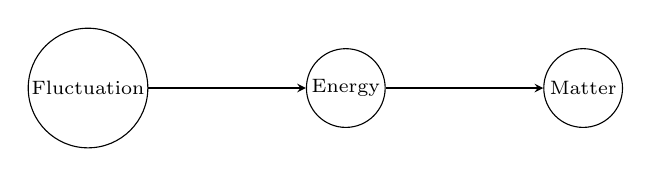
\begin{tikzpicture}[%
      node distance=2cm,
      scale=0.6,
      >=stealth,
      every node/.style={circle,draw,minimum size=1cm,inner sep=1pt,font=\scriptsize},
      every edge/.style={thick}
    ]
    \node (F) {Fluctuation};
    \node (E) [right=of F] {Energy};
    \node (M) [right=of E] {Matter};
    \draw[->] (F) -- (E);
    \draw[->] (E) -- (M);
  \end{tikzpicture}
  \caption{Causal flow from vacuum fluctuations to energy to matter.}
  \label{fig:dag}
\end{figure}

\subsection{Fractal Nesting Diagram}
\begin{figure}[htbp]
  \centering
  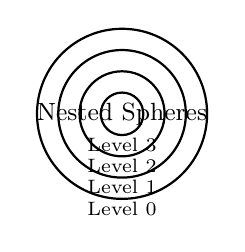
\begin{tikzpicture}[scale=0.6]
    \foreach \i/\r in {0/1.8,1/1.35,2/0.9,3/0.45} {
      \draw[thick] (0,0) circle (\r);
      \node at (0,-\r-0.2) {\scriptsize Level \i};
    }
    \node at (0,0) {\small Nested Spheres};
  \end{tikzpicture}
  \caption{Fractal nesting of spacetime spheres scaled by $\phi$.}
  \label{fig:fractal}
\end{figure}

%-------------------------------------------------------------------------------
\section{Applications}
\subsection{Cosmology}
Interdependent cycles predict enhanced cluster-scale lensing (\(\approx4\times\) standard)
and CMB multipole anomalies for \(\ell>2000\).

\subsection{Quantum Mechanics}
Vacuum fluctuations \(\to\) particle creation rates governed by
\(\Delta E\,\Delta t\ge\hbar\) under interdependence constraints.

%-------------------------------------------------------------------------------
\section{Testable Predictions}
\begin{itemize}
  \item \textbf{Gravitational Lensing:} \(\approx4\times\) stronger effective gravity in clusters.
  \item \textbf{CMB Anomalies:} Excess power at \(\ell>2000\) beyond \(\Lambda\)CDM.
  \item \textbf{LHC Bounds:} Deviations in cross-sections from fractal-spacetime corrections.
\end{itemize}

%-------------------------------------------------------------------------------
\section{Conclusion}
Dependent origination, formalized via vacuum wave-functions, Markov chains,
and golden-ratio fractals, yields a consistent, predictive framework unifying
quantum and cosmological phenomena.

%-------------------------------------------------------------------------------
\begin{acknowledgments}
We dedicate this work to Buddha Shakyamuni and all teachers of interdependence.
No external funding was used.
\end{acknowledgments}

%-------------------------------------------------------------------------------
\bibliographystyle{unsrt}
\begin{thebibliography}{9}
\bibitem{planck2018}
  Planck Collaboration, “Planck 2018 results. VI. Cosmological parameters,”
  \emph{Astron.\ Astrophys.}\ \textbf{641}, A6 (2020).

\bibitem{fractalbindu}
  A.~Preece, “Fractal Bindu Quantum Mechanics: The Manifestation of Reality’s Perfect Nature,”
  Independent Research (2025).

\bibitem{markov}
  J.~R.~Norris, \emph{Markov Chains}, Cambridge Univ.\ Press (1998).

\bibitem{hubble}
  E.~Hubble, “A Relation Between Distance and Radial Velocity Among Extra-Galactic Nebulae,”
  \emph{Proc.\ Natl.\ Acad.\ Sci.}\ \textbf{15}(3), 168–173 (1929).
\end{thebibliography}

\end{document}